% **************************************************
% Clean Thesis
% -- A LaTeX Style for Thesis Documents --
% 
% Copyright (C) 2011-2013 Ricardo Langner
% **************************************************
%
% Readme:
% ----------------------------------------
% *** Clean, Simple, Elegant ***
% "Clean Thesis" is a LaTeX style for thesis documents, developed
% for my diplom thesis (Diplomarbeit). The style can be understood
% as my personal compromise - a typical clean looking scientific
% document combined and polished with minor beautifications.
% 
% The design of this "Clean Thesis" style is inspired
% by user guide documents from Apple Inc.
% 
% Note: If you are looking for an exact and correct style regarding
% typographic rules, please have a look at the "Classic Thesis Style"
% (see http://www.miede.de/index.php?page=classicthesis).
% 
% *** Donation = Postcard ***
% Based on the idea of Andr\'e Miede: If you like the "Clean Thesis"
% style I would be very pleased about a donation in the form of a
% POSTCARD. You can find my address in the file Clean-Thesis.pdf.
% I am going to collect all postcards and exhibit them at the website
% I mentioned.
% 
% *** Idea and Inspiration ***
% The idea of providing my customized style for thesis documents
% passed through my mind while writing my own thesis. Motivated and
% inspired by the superb "Classic Thesis Style"
% (see http://www.miede.de/index.php?page=classicthesis) by Andr\'e Miede
% (thanks to Andr\'e for doing a great job) I decided to collect all
% design and style related functionality in a separate LaTeX style and
% provide this style to other thesis writers.
% 
% 
% License Information:
% ----------------------------------------
% "Clean Thesis" is free software: you can redistribute it and/or modify
% it under the terms of the GNU General Public License as published by
% the Free Software Foundation, either version 3 of the License, or
% (at your option) any later version.
% 
% "Clean Thesis" is distributed in the hope that it will be useful,
% but WITHOUT ANY WARRANTY; without even the implied warranty of
% MERCHANTABILITY or FITNESS FOR A PARTICULAR PURPOSE.  See the
% GNU General Public License for more details.
% 
% You should have received a copy of the GNU General Public License
% along with this program.  If not, see <http://www.gnu.org/licenses/>.
% **************************************************


% **************************************************
% Document Class Definition
% **************************************************
\documentclass[%
	paper=A4,					% paper size --> A4 is default in Germany
	twoside=false,				% onesite or twoside printing
	openright,					% doublepage cleaning ends up right side
	parskip=full,				% spacing value / method for paragraphs
	chapterprefix=true,			% prefix for chapter marks
	11pt,						% font size
	headings=normal,			% size of headings
	bibliography=totoc,			% include bib in toc
	listof=totoc,				% include listof entries in toc
	titlepage=on,				% own page for each title page
	captions=tableabove,		% display table captions above the float env
	draft=false,				% value for draft version
]{scrreprt}%

% **************************************************
% Debug LaTeX Information
% **************************************************
%\listfiles

% **************************************************
% Information and Commands for Reuse
% **************************************************
\newcommand{\thesisTitle}{Darwinian Networks Library}
\newcommand{\thesisName}{Andr\'e Evaristo dos Santos
\\ 
Jhonatan de Souza Oliveira
}
\newcommand{\thesisSubject}{Documentation}
\newcommand{\thesisDate}{August 10, 2015}
%\newcommand{\thesisVersion}{0.6.8}

%\newcommand{\thesisFirstReviewer}{Jane Doe}
%\newcommand{\thesisFirstReviewerUniversity}{\protect{Clean Thesis Style University}}
%\newcommand{\thesisFirstReviewerDepartment}{Department of Clean Thesis Style}
%
%\newcommand{\thesisSecondReviewer}{John Doe}
%\newcommand{\thesisSecondReviewerUniversity}{\protect{Clean Thesis Style University}}
%\newcommand{\thesisSecondReviewerDepartment}{Department of Clean Thesis Style}

\newcommand{\thesisFirstSupervisor}{Dr. Cory Butz}
%\newcommand{\thesisSecondSupervisor}{John Smith}

\newcommand{\thesisUniversity}{\protect{University of Regina}}
\newcommand{\thesisUniversityDepartment}{Department of Computer Science}
%\newcommand{\thesisUniversityInstitute}{Institut for Clean Thesis Dev}
%\newcommand{\thesisUniversityGroup}{Clean Thesis Group (CTG)}
\newcommand{\thesisUniversityCity}{Regina}
\newcommand{\thesisUniversityStreetAddress}{3737 Wascana Parkway}
\newcommand{\thesisUniversityPostalCode}{S4S 0A2}

% **************************************************
% Load and Configure Packages
% **************************************************
\usepackage[utf8]{inputenc}		% defines file's character encoding
\usepackage[english]{babel} % babel system, adjust the language of the content
\usepackage{marginnote} %margin note
\usepackage[					% clean thesis style
	figuresep=colon,%
	sansserif=false,%
	hangfigurecaption=false,%
	hangsection=true,%
	hangsubsection=true,%
	colorize=full,%
	colortheme=bluemagenta,%
	bibsys=bibtex,
]{cleanthesis}

\hypersetup{					% setup the hyperref-package options
	pdftitle={\thesisTitle},	% 	- title (PDF meta)
	pdfsubject={\thesisSubject},% 	- subject (PDF meta)
	pdfauthor={\thesisName},	% 	- author (PDF meta)
	plainpages=false,			% 	- 
	colorlinks=false,			% 	- colorize links?
	pdfborder={0 0 0},			% 	-
	breaklinks=true,			% 	- allow line break inside links
	bookmarksnumbered=true,		%
	bookmarksopen=true			%
}

% **************************************************
% Document CONTENT
% **************************************************
\begin{document}

% --------------------------
% rename document parts
% --------------------------
%\renewcaptionname{ngerman}{\figurename}{Abb.}
%\renewcaptionname{ngerman}{\tablename}{Tab.}
\renewcaptionname{english}{\figurename}{Fig.}
\renewcaptionname{english}{\tablename}{Tab.}

% --------------------------
% Front matter
% --------------------------
\pagenumbering{roman}			% roman page numbing (invisible for empty page style)
\pagestyle{empty}				% no header or footers
% !TEX root = ../thesis-example.tex
%
% ------------------------------------  --> cover title page
\begin{titlepage}
	\pdfbookmark[0]{Cover}{Cover}
	\flushright
	\hfill
	\vfill
	{\LARGE\thesisTitle} \par
	\rule[5pt]{\textwidth}{.4pt} \par
	{\Large\thesisName}
	\vfill
	\textit{\large\thesisDate} \\
%	Version: \thesisVersion
\end{titlepage}


% ------------------------------------  --> main title page
\begin{titlepage}
	\pdfbookmark[0]{Titlepage}{Titlepage}
	\tgherosfont
	\centering
	
%	{\Large \thesisUniversity} \\[4mm]
	
\includegraphics[width=6cm]{img/logo_uofr_black} \\[2mm]
	\textsf{\thesisUniversityDepartment} \\
%	\textsf{\thesisUniversityInstitute} \\
%	\textsf{\thesisUniversityGroup} \\
	
	\vfill
	{\LARGE \color{ctcolormain}\textbf{\thesisTitle} \\[10mm]}
	{\Large \thesisName} \\
	
	\vfill
%	\begin{minipage}[t]{.27\textwidth}
%		\raggedleft
%		\textit{1. Reviewer}
%	\end{minipage}
%	\hspace*{15pt}
%	\begin{minipage}[t]{.65\textwidth}
%		{\Large \thesisFirstReviewer} \\
%	  	{\small \thesisFirstReviewerDepartment} \\[-1mm]
%		{\small \thesisFirstReviewerUniversity}
%	\end{minipage} \\[5mm]
%	\begin{minipage}[t]{.27\textwidth}
%		\raggedleft
%		\textit{2. Reviewer}
%	\end{minipage}
%	\hspace*{15pt}
%	\begin{minipage}[t]{.65\textwidth}
%		{\Large \thesisSecondReviewer} \\
%	  	{\small \thesisSecondReviewerDepartment} \\[-1mm]
%		{\small \thesisSecondReviewerUniversity}
%	\end{minipage} \\[10mm]
%	\begin{minipage}[t]{.27\textwidth}
%		\raggedleft
%		\textit{Supervisors}
%	\end{minipage}
%	\hspace*{15pt}
%	\begin{minipage}[t]{.65\textwidth}
%		\thesisFirstSupervisor\ and \thesisSecondSupervisor
%	\end{minipage} \\[10mm]
	
	\thesisDate \\
	
\end{titlepage}


% ------------------------------------  --> lower title back for single page layout
\hfill
\vfill
\small
\textbf{\thesisName} \\
\textit{\thesisTitle} \\
\thesisDate \\
%Reviewers: \thesisFirstReviewer\ and \thesisSecondReviewer \\
Supervisor: \thesisFirstSupervisor\
%and \thesisSecondSupervisor 
\\[1.5em]
\textbf{\thesisUniversity} \\
%\textit{\thesisUniversityGroup} \\
%\thesisUniversityInstitute \\
\thesisUniversityDepartment \\
\thesisUniversityStreetAddress \\
\thesisUniversityPostalCode \thesisUniversityCity
		% INCLUDE: all titlepages
\cleardoublepage

\pagestyle{plain}				% display just page numbers
% !TEX root = Clean-Thesis.tex
%
\pdfbookmark[0]{Abstract}{Abstract}
\chapter*{Abstract}
\label{sec:abstract}
\vspace*{-10mm}

We propose a programming library for Darwinian networks (DNs).
The library covers adaptation and evolution in DNs, for modelling a problem domain and inference on the model, respectively.
The implementation uses C++, expanding over a well established BN library called aGrUM.
Furthermore, a wrapper in Python is created over the C++ library, in order to facilitate the development of DN systems with a scripting language.
		% INCLUDE: the abstracts (english and german)
\cleardoublepage
%
%% !TEX root = ../thesis-example.tex
%
\pdfbookmark[0]{Acknowledgement}{Acknowledgement}
\chapter*{Acknowledgement}
\label{sec:acknowledgement}
\vspace*{-10mm}

\Blindtext[2][2]
 % INCLUDE: acknowledgement
%\cleardoublepage
%
\setcounter{tocdepth}{2}		% define depth of toc
\tableofcontents				% display table of contents
\cleardoublepage

% --------------------------
% Body matter
% --------------------------
\pagenumbering{arabic}			% arabic page numbering
\setcounter{page}{1}			% set page counter
\pagestyle{maincontentstyle} 	% fancy header and footer

% !TEX root = ../thesis-example.tex
%
\chapter{Introduction}
\label{sec:intro}

\cleanchapterquote{In the long history of humankind (and animal kind, too) those who learned to collaborate and improvise most effectively have prevailed.}{Charles Darwin}{}

Darwinian networks (DNs) \cite{butzOliveiraSantosCai15} were proposed as a simplification of working with Bayesian networks (BNs).
A BN is a set of \emph{conditional probability tables} (CPTs) and a \emph{direct acyclic graph} (DAG) \cite{pear88}.
The DAG is used to represent graphically the relations between vertices and each vertex is associate with a CPT that quantifies those reslations.
On the other hand, a DN directly draws the CPTs as a dashed circle called population.
A population has white and black nodes, called combative and docile traits, respectively.
Combative traits are used to represent variables on the LHS of a CPT and docile traits represent the variables of the RHS of a CPT.
Therefore, a DN is defined as a multi-set of populations.

Modeling in BNs involves testing independencies in a DAG using a graphical test called \emph{d-separation} \cite{pear88}.
Testing independencies in DNs can be graphically performed with a test called \emph{adaptation} \cite{butzOliveiraSantosCai15}.
Inference in BN is done by systematically manipulating the CPTs with multiplications and divisions and marginalization.
DNs graphically represents multiplications and divisions with the merge of populations and marginalization with replication of populations followed by natural selection.
DNs perform both modeling and inference in the same platform.

A programming library is essential to run experimental results, develop real world systems, incentive the literature in the area, among other applications.
In this project, we propose the implementation of a DN library, which contains the basic tools for modeling, testing adaptation and performing evolution in DNs.
A user of the library can work with DNs following general ideas from published papers in DNs \cite{butzOliveiraSantosCai15} and discover new practical understanding of BNs, all applied with simple procedures that act with the same remarkable robust view of DNs.

For modeling DNs, the library makes available procedures for all steps of adaptation, first defining populations with combative and docile traits.
Then, to test adaptation between two sets of populations ${\cal P}_X$ and ${\cal P}_Z$ given a third set of populations ${\cal P}_Y$, namely $A({\cal P}_X, {\cal P}_Y, {\cal P}_Z)$, it is simply necessary to define an initial and a final DN.
Moreover, the process of natural selection removes barren populations and the procedure for docilization acts on the resulting DN adding docile populations (populations containing only docile traits) for each population with more than one docile trait.
Deletion procedure then removes all populations in ${\cal P}_Y$.
Finally, a procedure for recursive merging is called in order to check if traits from ${\cal P}_X$ and ${\cal P}_Z$ end up together in a same population.

For inference, three basic procedures are available, namely, merge, replication and natural selection.
First, an initial and final DNs are determined.
The merge of two populations combines them into a new population with all combative traits and some of the docile traits.
When two combative traits for the same variable occurs that means a division.
The library is capable to detect all the possible combination of traits and perform the respective operation.
Replication of a population is a procedure which makes a copy of that population in the current DN as well as generated any other population with all the docile from the original one but a subset of the combative traits.
Then, natural selection can be called eventually in order to remove unnecessary populations for that evolution up to when the call occurs.

The implementation of the DN library utilizes Python programming language, known for its code readability and simple syntax.
As a base for DN library, we develop a reliable framework for probabilistic graphical models, called \emph{Darwin Library}, that is, all the basic data structure such as CPTs, potentials, variables, multiplication, addition, and division are used from Darwin Library.
Besides of the reliable implementation of Darwin Library, another advantage of using this framework is to provide a platform for fair comparison between BNs and DNs, since both are in the same programming language and the same set of basic implementation.
One salient feature of Darwin library it is test unity for all its operation classes.
A test unity is a software testing method which uses individual units of source code that are tested to determine whether they are fit for use \cite{kolawa2007automated}.
The DN library will also use \emph{IPython Notebook} \cite{PER-GRA:2007} in order to provide a Python programming interface for the users.

%to finish
In summary, this project proposes the implementation of a DN library.
All the basic operations for adaptation and evolution in DNs is available through the library.
The implementation itself uses Python programming language and the basic data structures are provided by Darwin library.
A Python interface will be also available for rapid prototyping systems and teaching.
The main advantage of the DN library is to apply novel ideas and techniques of DNs that were recently propose to simplify working with BNs.

 % INCLUDE: introduction
\chapter{Background}
\label{sec:background}

\reversemarginpar

We review modeling and inference in BNs and in DNs.

\section{Bayesian Networks}
\label{sec:baysian_networks}

Let $U = \{ v_1, v_2, \ldots , v_n \}$ be a finite set of variables, each with a finite domain.
A singleton set $\{v\}$ may be written as $v$, $\{ v_1, v_2, \ldots, v_n \}$ as $v_1 v_2 \cdots v_n$, and $X \cup Y$ as $XY$.
For disjoint $X,Y \subseteq U$, a \emph{conditional probability table} (CPT) $P(X|Y)$ is a potential over $XY$ that sums to one for each value $y$ of $Y$.
The \emph{children} $Ch(v_i)$ and \emph{parents} $Pa(v_i)$ of $v_i$ are those $v_j$ such that $(v_i,v_j) \in \cal{B}$ and $(v_j,v_i) \in \cal{B}$, respectively.

A \emph{Bayesian network}\marginnote{\tiny BAYESIAN NETWORK} (BN) \cite{pear88} is a \emph{directed acyclic graph} (DAG) $\cal{B}$ on $U$ together with CPTs $P(v_1 | Pa(v_1))$, $P(v_2|Pa(v_2)),$$\ldots,$ $P(v_n|Pa(v_n))$, where the \emph{parents} $Pa(v_i)$ of $v_i$ are those $v_j$ such that $(v_j,v_i) \in \cal{B}$.
We call $\cal{B}$ a BN, if no confusion arises.
Figure \ref{fig:dag} shows a BN with CPTs $P(fo)$, $P(bp)$, $P(lo|fo)$, $P(do|bp,fo)$, and $P(hb|do)$ shown.

\begin{figure}[hbt]
    \begin{center}
        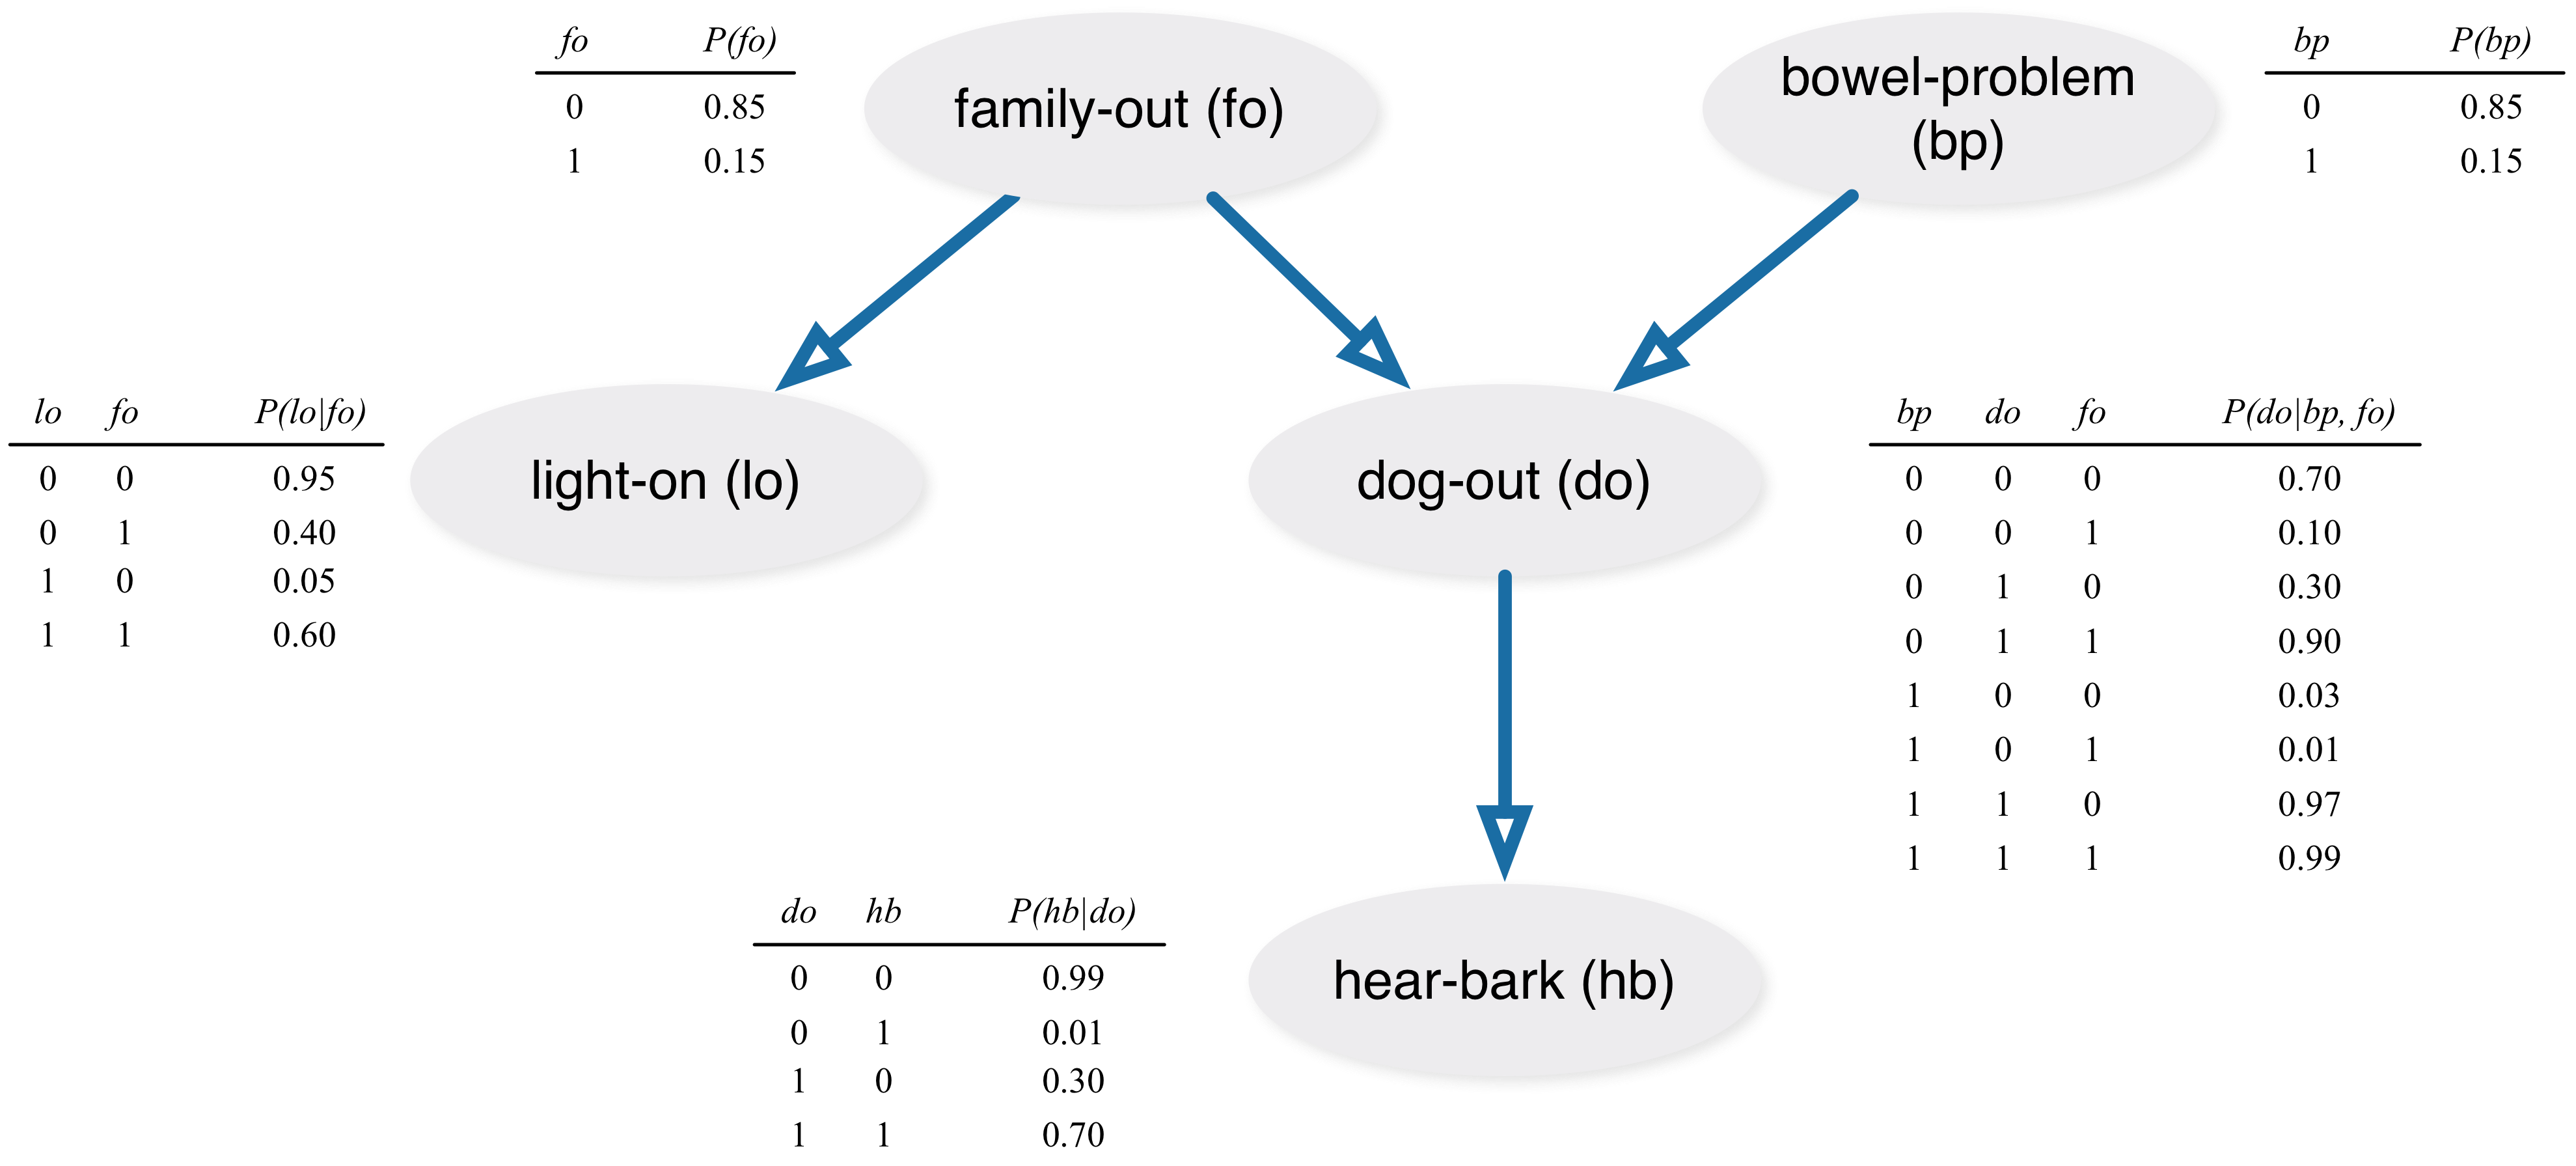
\includegraphics[width=\textwidth]{img/DAG_darwiche}
    \end{center}
    \caption{A DAG ${\cal B}$ and its CPTs from \cite{darwiche09}.}
    \label{fig:dag}
\end{figure}

The \emph{conditional independence} \cite{pear88} of $X$ and $Z$ given $Y$ holding in $P(U)$ is denoted $I(X,Y,Z)$.
The \emph{d-separation method}\marginnote{\tiny D-SEPARATION} \cite{pear88} can be used to read independencies from a DAG.
It is known that if $I_{\cal{B}}(X,Y,Z)$ holds by d-separation in ${\cal B}$, then $I(X,Y,Z)$ holds in $P(U)$.

One method to perform inference on a DAG is called \emph{Variable elimination}\marginnote{\tiny VARIABLE ELIMINATION} (VE) \cite{zhan94}, which computes $P(X|Y=y)$ from a BN $\cal{B}$ as follows:
(i) all barren variables are removed recursively, where $v$ is \emph{barren} \cite{zhan94}, if $Ch(v) = \emptyset$ and $v \not\in XY$;
(ii) all independent by evidence variables are removed, giving ${\cal{B}}^s$, where $v$ is an \emph{independent by evidence} variable, if $I(v,Y,X)$ holds in $\cal{B}$ by m-separation;
(iii) build a uniform distribution $1(v)$ for any root of ${\cal{B}}^s$ that is not a root of $\cal{B}$;
(iv) set $Y$ to $Y=y$ in the CPTs of ${\cal{B}}^s$;
(v) determine an elimination ordering $\sigma$ from the moral graph ${\cal{B}}^{s}_{m}$ (as explained later);
(vi) following $\sigma$, eliminate variable $v$ by multiplying together all potentials involving $v$, and then summing $v$ out of the product;
and, (vii) multiply together all remaining potentials and normalize to obtain $P(X|Y=y)$.


To perform probabilistic inference, a BN is commonly transformed into a \emph{Markov network} \marginnote{\tiny MARKOV NETWORK}(MN) \cite{pear88}, also called a \emph{decomposable} MN. 
A MN consists of a triangulated (chordal) graph together with a potential defined over each maximal clique of triangulated graph. 
Given a DAG, the \emph{moralization} \cite{laur88} of the DAG is the undirected graph constructed by adding an undirected edge between each pair of parents of a common child and then dropping directionality.
When necessary, edges are added to the moralized graph to obtain a triangulated graph. 
The maximal cliques are organized as join tree $\cal T$. 
Finally, the CPTs of the BN are assigned to nodes of $\cal T$. 


%\clearpage

\section{Darwinian Networks}
\label{sec:darwinian_networks}

\emph{Darwinian networks} (DNs)\marginnote{\tiny DARWINIAN NETWORKS} \cite{butzOliveiraSantosCai15} were proposed to simplify working with \emph{Bayesian networks} (BNs) \cite{pear88}.
Rather than modeling the variables in a problem domain, DNs represent the probability tables in the model.
The graphical manipulation of the tables then takes on a biological feel, where a CPT $P(X|Y)$ is viewed as the novel representation of a \emph{population} $p(C,D)$ using both \emph{combative} traits $C$ (coloured clear) and \emph{docile} traits $D$ (coloured dark).

\begin{figure}[hbt]
    \begin{center}
        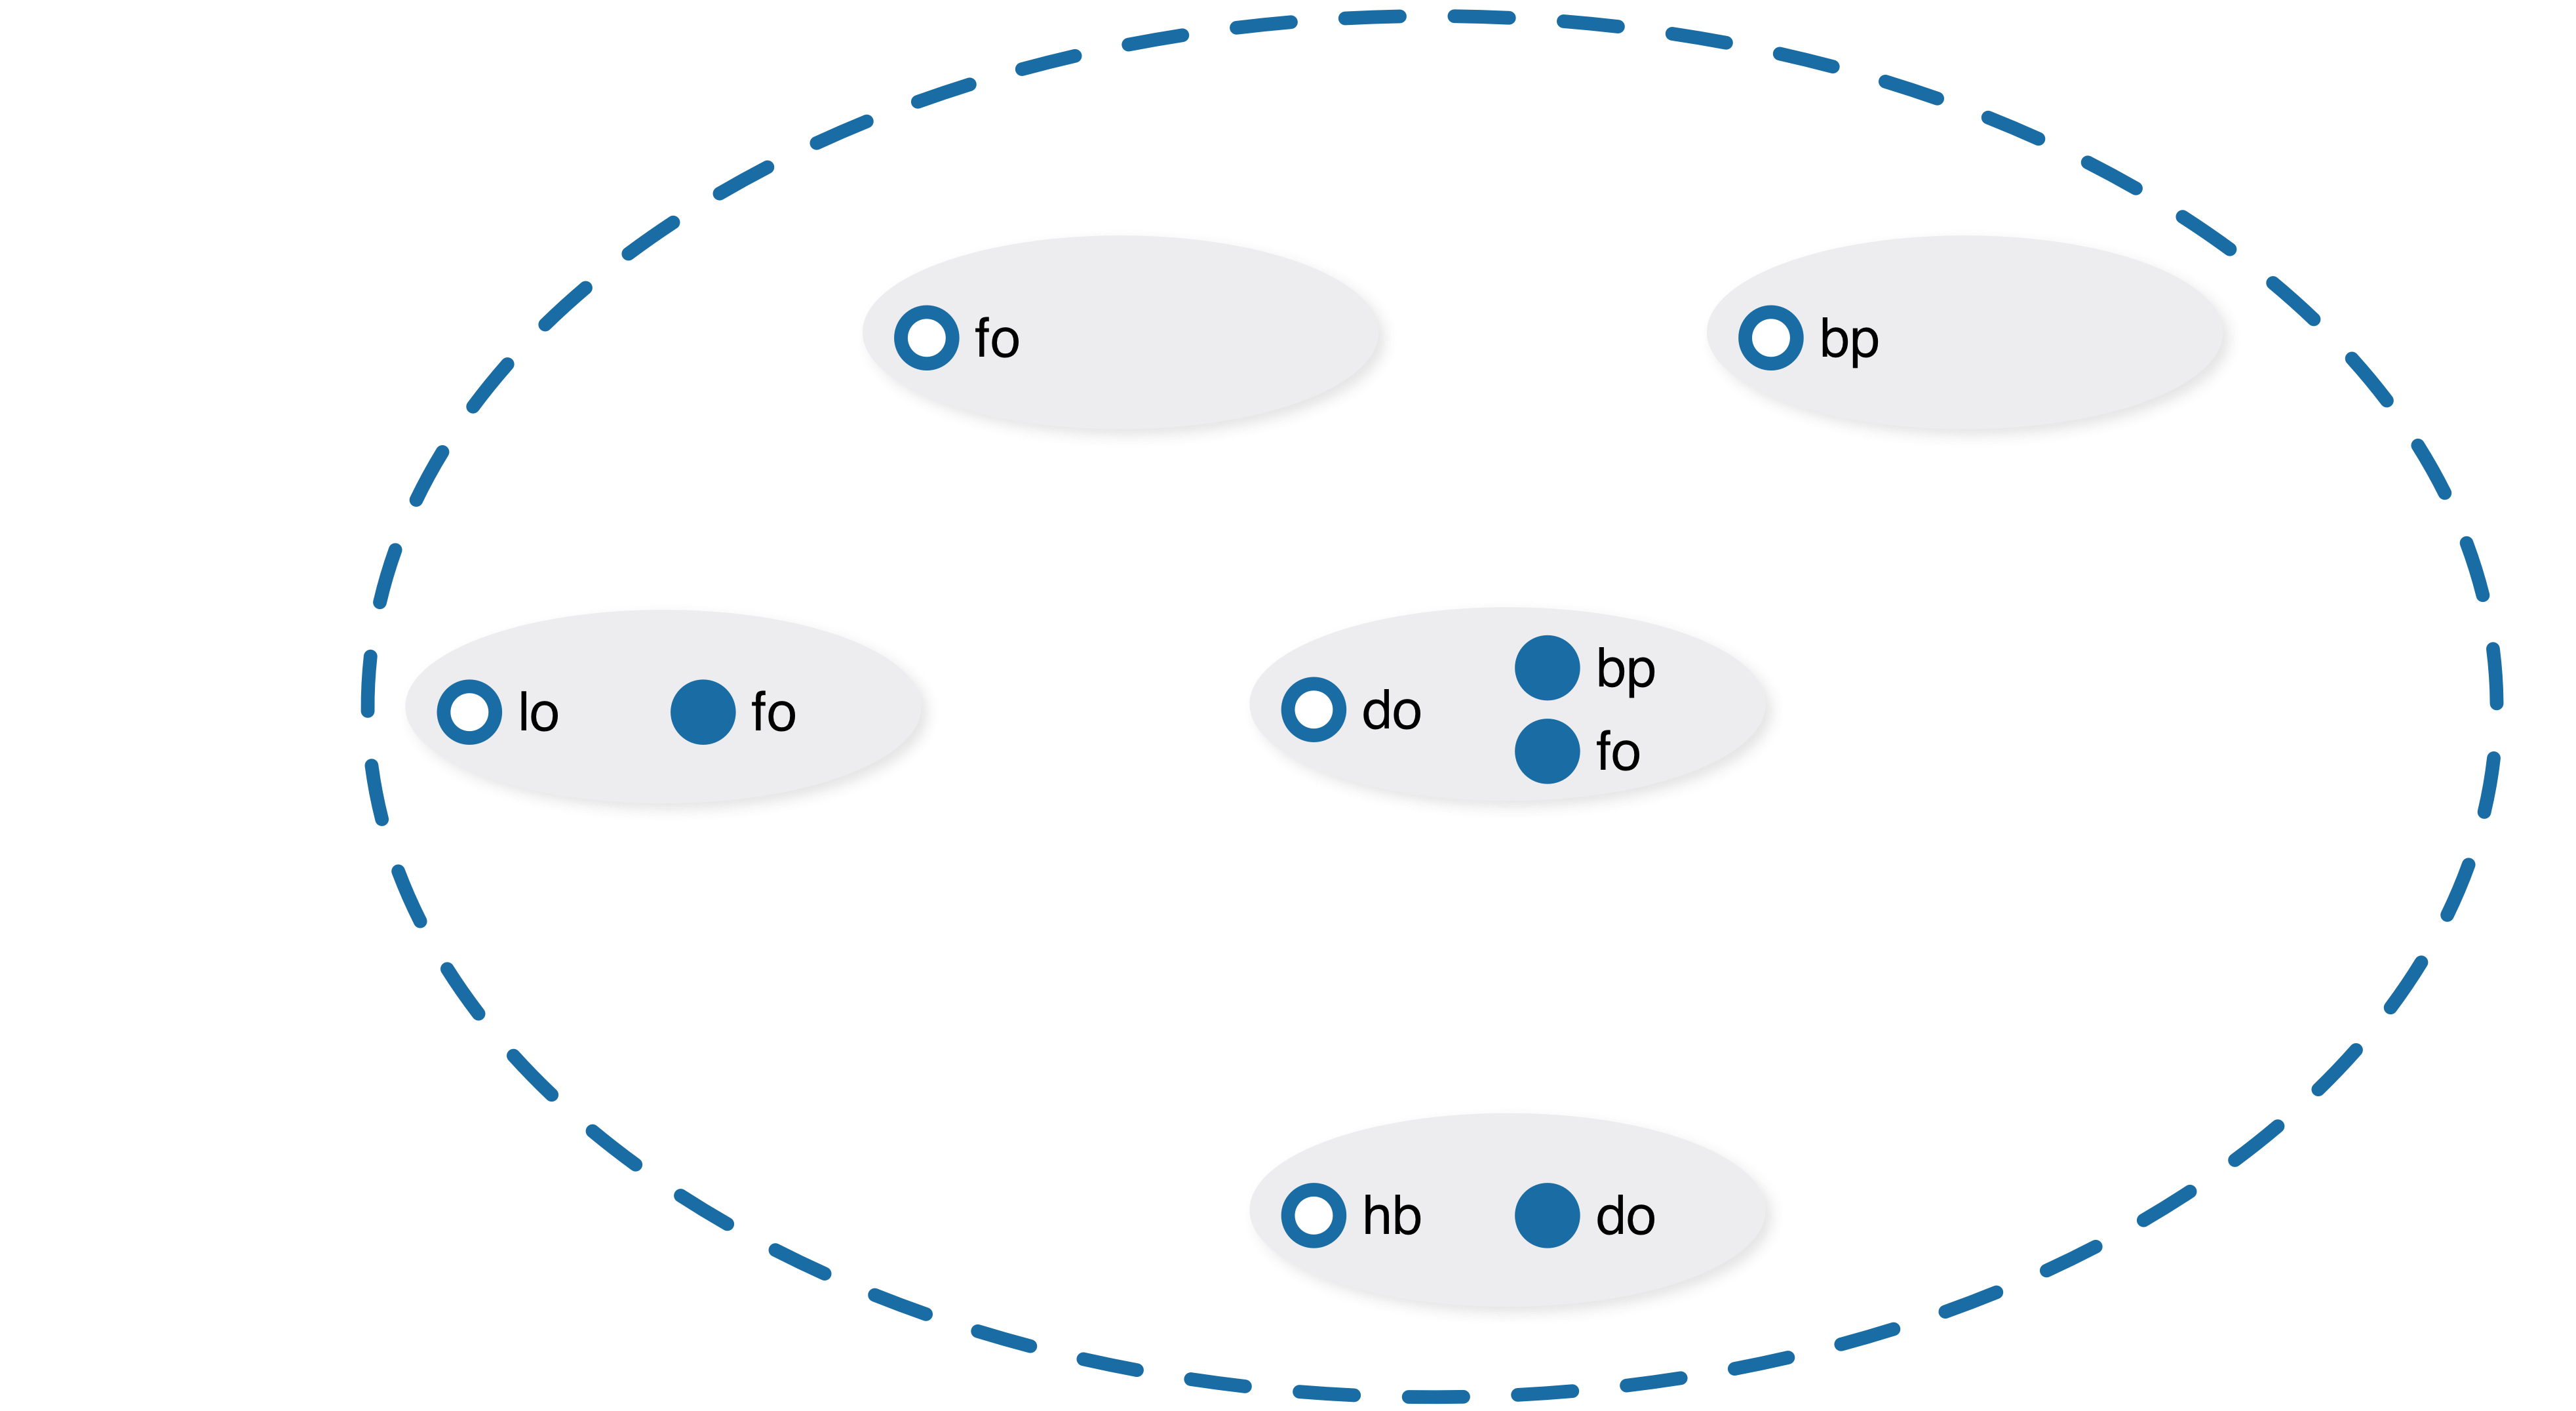
\includegraphics[width=\textwidth]{img/DN_darwiche}
    \end{center}
    \caption{A DN ${\cal D}$ representing DAG ${\cal B}$ of Figure \ref{fig:dag}.}
    \label{fig:dn}
\end{figure}

Adaptation and evolution are used to represent the testing of independencies and inference, respectively.
Thus, DNs can represent exact inference VE, as well the test of independencies d-separation.
Hence, DNs can unify modeling and reasoning tasks into a single platform.
The query $P(X|Y)$ posed to a BN ${\cal B}$ is represented by DN ${\cal D}^{\prime} = \{ p(X,Y) \}$ and the test of independence $I_{\cal{B}}(X,Y,Z)$ holds in a BN $\cal{B}$ if and only if tha adaptation $A({\cal{P}}_X, {\cal{P}}_Y, {\cal{P}}_Z)$ succeeds in the DN $\cal{D}$ for $\cal{B}$.



\subsection{Definitions}
\label{subsec:definitions}


%TRAIT

		A \emph{trait}\marginnote{\tiny TRAIT} $t$ can be combative or docile.
		A \emph{combative} trait $t_c$ is depicted by a clear (white) circle.
		A \emph{docile} trait $t_d$ is illustrated by a dark (black) circle.

%POPULATION

		A \emph{population}\marginnote{\tiny POPULATION}  $p(C,D)$ contains a non-empty set $CD$ of traits, where $C$ and $D$ are disjoint, $C$ is exclusively combative, and $D$ is exclusively docile.
		A population is depicted by a closed curve around its traits.

%DN

		A \emph{Darwinian network} (DN)\marginnote{\tiny DN} , denoted $\cal{D}$, is a finite, multiset of populations.
		A DN $\cal{D}$ is depicted by a dashed closed curve around its populations.
		All combative traits in a given DN $\cal{D}$ are defined as $T_c(\cal{D})$ $=$ $\{t_{c} ~ | ~ t_{c} \in C,$ for at least one $p(C,D) \in \cal{D}\}$.
		All docile traits in $\cal{D}$, denoted $T_d(\cal{D})$, are defined similarly


\subsection{Operations}
\label{subsec:operations}



%		DOCILIZATION
		
		\emph{Docilization}\marginnote{\tiny DOCILIZATION} of a DN $\cal{D}$ adds $p(\emptyset,D)$ to $\cal D$, for every population $p(C,D)$ in ${\cal D}$ with $|D| > 1$.
		

%		DELETION
		
		To \emph{delete}\marginnote{\tiny DELETION} a population $p(C,D)$ from a DN $\cal{D}$ is to remove all occurrences of it from $\cal{D}$.
		

%		MERGE
		
		Two populations \emph{merge}\marginnote{\tiny MERGE} together as follows: for each trait $t$ appearing in either population, if $t$ is combative in exactly one of the two populations, then $t$ is combative in the merged population; otherwise, $t$ is docile.
		

%		NATURAL SELECTION
		
		In adaptation, \emph{natural selection}\marginnote{\tiny NATURAL SELECTION} removes recursively all barren populations from a DN $\cal{D}$ with respect to another DN ${\cal{D}}^{'}$.
		

%		REPLICATION
		
		\emph{Replication}\marginnote{\tiny REPLICATION} of a population $p(C,D)$ gives $p(C,D)$, as well as any set of populations $p(C^{'}, D)$, where $C^{'} \subset C$.
		

\subsection{Modeling}
\label{subsec:adaptation}


In DNs, how populations ``adapt'' to the deletion of other populations corresponds precisely with testing independencies in BNs.

Let ${\cal{P}}_X$, ${\cal{P}}_Y$, and ${\cal{P}}_Z$ be pairwise disjoint subsets of populations in a DN $\cal D$ and let DN ${\cal{D}}^{'} = {p(C)}$, where $C = T_c({\cal{P}}_X {\cal{P}}_Y {\cal{P}}_Z)$. 
The test \emph{adaptation}\marginnote{\tiny ADAPTATION} of ${\cal{P}}_X$ and ${\cal{P}}_Z$ given ${\cal{P}}_Y$, denoted $A({\cal{P}}_X,{\cal{P}}_Y,{\cal{P}}_Z)$, in $\cal D$ with four simple steps:
(i) let natural selection act on $\cal{D}$ with respect to ${\cal{D}}^{'}$, giving ${\cal{D}}^{s}$;
(ii) construct the docilization of ${\cal{D}}^{s}$, giving ${\cal{D}}^s_m$;
(iii) delete $p(C,D)$ from ${\cal{D}}^s_m$, for each $p(C,D)$ in ${\cal{P}}_Y$; and,
(iv) after recursively merging populations sharing a common trait, if there exists a population containing both a combative trait in $T_c({\cal{P}}_X)$ and a combative trait in $T_c({\cal{P}}_Z)$, then $A({\cal{P}}_X,{\cal{P}}_Y,{\cal{P}}_Z)$ fails; otherwise, $A({\cal{P}}_X,{\cal{P}}_Y,{\cal{P}}_Z)$ succeeds.


\subsection{Inference}
\label{subsec:evolution}


The \emph{evolution}\marginnote{\tiny EVOLUTION} of a DN $\cal{D}$ into a DN ${\cal{D}}^{'}$ occurs by natural selection removing recursively all barren, independent, and spent populations, merging existing populations, and replicating to form new populations.


 % INCLUDE: related work
\chapter{Darwin Library}
\label{sec:darwin_lib}

Darwin is a simple library written in Python for BN modelling and inference.
The main purpose of the library is teaching and quick prototyping or testing.
In order to achieve these goals, the library has a simplistic approach of implementation, using native Python data structure and light usage of object oriented programming.
The structure of Darwin is basically divided into two categories: potentials and graph manipulations.
The features are also split into two main categories: tools for inference and modelling.
Furthermore, in this section we also present a guide for getting started using Darwin.

\section{Structure}
\label{sec:system:sec1}

In order to work with BNs, Darwin has two main set of implementations: potential and graph manipulations.
These two categories form individually or together the tree structure of the library as presented in Figure \ref{fig:tree_darwin}.

\begin{figure}[hbt]
    \begin{center}
        
\includegraphics[width=0.6\textwidth]{img/logo_uofr_black}
    \end{center}
    \caption{Three structure of Darwin.}
    \label{fig:tree_darwin}
\end{figure}


At the root, the class \emph{Potential} is a data structure for modelling a probability table.
The \emph{NetworkX} is set of data structures for graph manipulation and is also included at the root of the library.
Similarly, \emph{GraphWithPotential} is a class which basically maps nodes in a graph with a set of potentials, besides providing manipulations on the graph and the potentials on it.
\emph{BayesianNetwork} is a class that inherits from \emph{GraphWithPotential} but maps only one potential per node.
This data structure is used for a BN modelling.
In the same way, the class \emph{MarkovNetwork} entirely inherits the behaviour and properties of \emph{GraphWithPotential}, therefore it can be used for MN modelling.

The \emph{Utils} branch is formed by a set of standalone functions which implement core procedures for the other classes.
Mainly, these functions are defined by numerical operations and can be optimized separately.
One advantage of having those implementations as standalone functions is that future optimized code can be included or modified without disturbing the other classes.
Basically, there are three main utilities: \emph{BnUtils}, \emph{MnUtils}, and \emph{PotentialUtils}.
The BnUtils has a set of functions for BN manipulations and operations, such as moralization, triangulization, join tree construction, among others.
In MnUtils, we have utilities for MN propagation such as finding a optimal path for propagating in a tree.
Lastly, PotentialUtils is formed by a set of procedures for numerical operations such as multiplication, division and marginalization of tables.
All potential manipulations in PotentialUtils is implemented according to the efficient implementation proposed in \cite{koll09}.

In the \emph{Modelling} brach, there is an implementation of d-Separation as proposed in Algorithm 3.1 of \cite{koll09}.
While in the branch \emph{Inference} there are few data structures useful for exact inference in BNs.
The \emph{Barren} function is used for identifying barren potentials in factorizations.
\emph{SumOut} is a function which systematically remove a set of variables from a factorization.
The class \emph{VariableElimination} implements the exact inference algorithm VE as originally proposed by \cite{zhan94}.
Finally, the \emph{Test} branch has a set of unit tests which assure the correct functioning of core functions in the whole library.

\section{Features}
\label{sec:system:sec2}

Here, we highlight some feature of the library.
In general, the features are tools to facilitate the use of Darwin in teaching and prototyping of small system.
The library is not intended for fast inference, neither high accuracy.
Therefore, all numerical operations are implemented using native Python code, instead of high performance libraries such as \emph{numpy}.
The graph manipulations are done by an external library called \emph{NetworkX}, a robust and well known library with high performance and large set of tools.

For modelling, Darwin has the testing of d-Separation implemented using a reachability algorithm.
Also, the library has built in tools for converting a BN into a MN, including the join tree construction by moralization, triangulization and the assignment of potentials.
The triangulization step, specifically, has implemented 4 different heuristics, the same as implemented in \emph{PgmPy}.

For inference, the library provides a basic function for eliminating variables in a factorization, called \emph{SumOut}.
But for faster inference, it is recommended to use the VE implementation which absorb evidence, removes barren and independent by evidence potentials, perform inference and, finally, normalize the final result.

\section{Usage}
\label{sec:system:sec3}

In order to get started with Darwin, we now present a quick overview of the most common classes and functions.
The main classes are \emph{Potential}, \emph{GraphWithPotential}, \emph{BayesianNetwork}, and \emph{MarkovNetwork}.

The Potential class is defined by the given arguments: \emph{variables} which is a list with strings, \emph{cardinalities} corresponding to the variables which is a list with integers in the same order than the variables, probabilities \emph{values} in a list with floating numbers, \emph{left hand side} which is a list with the variables in the LHS of the potential, and similarly the \emph{right hand side} is defined.
For example, considering a CPT $P(a|b)$ with binary variables and probability values 0.4, 0.5, 0.6, 0.5, we can use Darwin to represent this potential as:
\begin{verbatim}
    Potential(["a", "b"], [2, 2], [0.4, 0.5, 0.6, 0.5], ["b"], ["a"])
\end{verbatim}

The GraphWithPotential class contains basically a list with potentials, a graph defined using NetworkX, and a dictionary mapping nodes in the graph to a list of potentials.
After declaring a GraphWithPotential, the user can add potentials to a node using the \emph{add\_potential} method.
For example, the following code creates a graph with two nodes $\{a\}$ and $\{a,b\}$ and assign $P(a)$ to $\{a\}$ and $P(b|a)$ to $\{a,b\}$ in a GraphWithPotential.
\begin{verbatim}
    p1 = Potential(["a"], [2], [0.2, 0.8], ["a"], [])
    p2 = Potential(["a", "b"], [2, 2], [0.4, 0.5, 0.6, 0.5], ["b"], ["a"])
    
    G = networkx.Graph()
    G.add_nodes(["a", "ab"])
    
    GwP = GraphWithPotential()
    GwP.add_potential("a", p1)
    GwP.add_potential("ab", p2)
\end{verbatim}

The MarkovNetwork inherits from GraphWithPotential, therefore modelling a MN is simply using the GraphWithPotential like in the code above.
In the same way, modelling a BN uses the BayesianNetwork class which also inherits from GraphWithPotential.
The difference for a BN is that only one potential is assigned at one node and the graph used is a DAG.
For instance, the code above can be used to declare a BN with two nodes $a \rightarrow ab$ just by changing the definition of $G$ to the below code, which is a directed graph.
\begin{verbatim}
    G = networkx.DiGraph()
    G.add_edge("a", "ab")
\end{verbatim}
	% INCLUDE: system
\chapter{Darwinian Network Library}
\label{sec:dn_lib}

\section{Structure}
\label{sec:system:sec1}

The DN library is a simple extension of Darwin, also intended for teaching and prototyping purposes.
Basically, the library inherits the potential manipulation tools from Darwin, ignoring the graphical manipulation ones.
From there, DN library builds the analysis of set of potentials, which forms a DN by definition.
The structure of the library is mainly formed by two classes: \emph{Population} and \emph{DarwinianNetwork}.

The Population class inherits directly from Potential's class in Darwin.
But here, few keywords are override in order to adapt the language for DNs.
For instance, the left and right hand side of the arguments in a Potential are called combative and docile in a Population.
Moreover, a Population have the methods merge and replicate which internally calls multiply (or divide) and marginalize from Potential.
Deciding where it is a division or multiplication is handled internally by the merge method.

DarwinianNetworks is defined with a set of Populations.
This data structure basically offers common methods for set manipulations, for instance, inserting and removing Populations.
Here, the set of populations are stored in an array, in order to allow the multiset populations as defined in DNs.

\section{Features}
\label{sec:system:sec2}

Few features are present in DN library in order to guarantee a smooth use for teaching and prototyping.
Now, we highlight there features of the library: keyword usage, initialization of parameters and drawing of data structure.

When instantiating a Population, the user can use keywords for the combative and docile arguments.
In this way, the user does not need to remember the ordering of the arguments, but only their names.
For example, defining a population $p(a,b)$ can be defined with the below code by using keywords ``combative'' and ``docile'':
\begin{verbatim}
    Population(combative=["a"],docile=["b"])
\end{verbatim}

Also for simplifying usage, the library has standard initialization of internal parameters.
That is, if the user does not pass all the required arguments, the DN library initialize them correctly when possible with standard values.
For example, in the above code the cardinalities of variables ``a'' and ``b'' are set to 2 and the 4 probabilities values are randomly generated between 0 and 1.

Finally, the DN library has a set of procedures for drawing Populations and DarwinianNetworks whenever the user calls them.
Those tools are built using the \emph{matplotlib} \cite{Hunter:2007} library for Python and is the only requirement for the drawings.
If the user wants to see how a population looks like, the user can define the Population and then calls the \emph{draw\_population} function as illustrate below:
\begin{verbatim}
    p = Population(combative=["d"],docile=["f", "b"])
    draw_population(p)
\end{verbatim}
These commands will create a drawing of a population as illustrated in Figure \ref{fig:drawing_pop}.

\begin{figure}[hbt]
    \begin{center}
        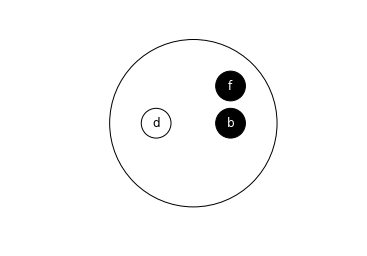
\includegraphics[width=0.6\textwidth]{img/drawing_population.png}
    \end{center}
    \caption{Drawing of population $p(d,fb)$ created by the DN library.}
    \label{fig:drawing_pop}
\end{figure}

The same idea works for a whole DN.
After defining a DarwinianNetwork, the user can call \emph{draw\_dn} passing the DN object.
Figure \ref{fig:drawing_dn} shows one example of the drawing of a DN as generated by the DN library.

\begin{figure}[hbt]
    \begin{center}
        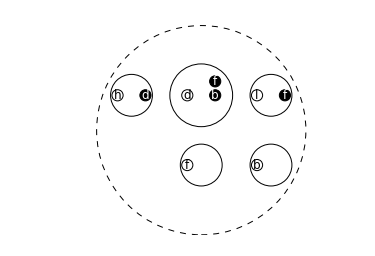
\includegraphics[width=0.6\textwidth]{img/drawing_dn.png}
    \end{center}
    \caption{Drawing of the DN $\{p(h,d), p(l,f), p(f), p(b), p(d,fb)\}$ created by the DN library.}
    \label{fig:drawing_dn}
\end{figure}

\section{Usage}
\label{sec:system:sec3}

The use of the two main classes in DN library is introduced now.
The Population class is defined exactly like a Potential, since it inherits from that class.
But the left and right hand side argument names are replaced by combative and docile, respectively.
Two methods are also exposed for quick references: combative and docile, which returns the respective informations for that Population.
A helper method called \emph{from\_potential} is also available in order to convert a Potential object to a Population one.
Moreover, merge receives another Population as argument, while replicate receives a list of variables which will be marginalized from the Population.

The DarwinianNetwork class has a list member where all the Populations are hold.
The methods \emph{add\_population} and \emph{delete\_population} are used for adding and deleting Population, respectively, from the list of Populations
This class has no constructor and the list of Populations is used to simulate the multi-set definition of DNs.
 % INCLUDE: concepts
\chapter{Applications}
\label{sec:application}

Three applications of the libraries

\section{Adaptation Tutorial}
\label{sec:conclusion:sec1}

\section{Evolution Tutorial}
\label{sec:conclusion:sec1}

\section{Test Unit}
\label{sec:conclusion:sec1}
 % INCLUDE: concepts
\chapter{Conclusion}
\label{sec:conclusion}

We proposed Darwinian Network Library as new framework for modeling and inference in DNs.
DN library is a implementation of the basic operations for adaptation and evolution in DNs.
It is implemented with the Python programming language and the basic data structures are provided by Darwin library.
%It provides salient features as test unity and a tutorials with IPython Notebook.
The main advantage of the DN library is to apply novel ideas and techniques of DNs.
DN library also is great for teaching, quick prototyping with DNs and testing.


DN library is based upon the novel library Darwin, a Python framework for BN modeling and inference.
Darwin library has two main categories called potentials and graph manipulations.
The former is a data structure for modeling a probability table.
The latter maps nodes in the graph to a list of potentials.
Together they form a reliable structure to reason on BNs.

We have established in Chapter \ref{sec:dn_lib} features of DN library given the manipulation tools from Darwin.
We have shown that DN library is an intuitive framework for working with DNs.
For instance, to build a set of potentials, one can simply utilize the class \emph{Population}.
Intuitively, with objects \emph{Population} together we can obtain a class \emph{DarwinianNetwork}.

Another salient feature is the set of procedures for drawing Populations and DarwinianNetworks.
It allows the user to see how looks like a population that has just been created - or even the entire DN!


This project proposes the implementation of a DN library.
In summary, we have stablished four main advantages of using DN library:
\begin{inparaenum}[(i)]
\item due its simple approach given the Python implementation, it has an expressive language that facilitate its usage;
\item it has interactive visual tools to compute and draw DNs, enabling users to better interact with the library;
\item it is a great tool for learning and its operations are sound given the unit tests;
\item and all source code is available free online on \emph{GitHub} through the webpage:
\end{inparaenum}
\begin{center}
\url{https://github.com/Darwinian-Networks}
\end{center}
With DN library, DNs can be applied as the simple and yet remarkably robust tool they are, allowing users to simplify reasoning with BNs.
 % INCLUDE: conclusion
\cleardoublepage

% --------------------------
% Back matter
% --------------------------
%{%


%\setstretch{1.1}
%\renewcommand{\bibfont}{\normalfont\small}
%\setlength{\biblabelsep}{0pt}
%\setlength{\bibitemsep}{0.5\baselineskip plus 0.5\baselineskip}
%\nocite{*}
%\printbibliography[nottype=online]
%\printbibliography[heading=subbibliography,title={Webseiten},type=online,prefixnumbers={@}]
%}
%\cleardoublepage

\bibliographystyle{splncs03}
\bibliography{references}


%\listoffigures
%\cleardoublepage
%
%\listoftables
%\cleardoublepage
%
%% !TEX root = ../thesis-example.tex
%
\pagestyle{empty}
\hfill
\vfill
\pdfbookmark[0]{Colophon}{Colophon}
\section*{Colophon}

This thesis was typeset with \LaTeXe.
It uses the \textit{Clean Thesis} style developed by Ricardo Langner.
The design of the \textit{Clean Thesis} style is inspired by user guide documents from Apple Inc.

Download the \textit{Clean Thesis} style at \url{http://cleanthesis.der-ric.de/}.

%\cleardoublepage
%
%% !TEX root = ../thesis-example.tex
%
%************************************************
% Declaration
%************************************************
\pdfbookmark[0]{Declaration}{Declaration}
\chapter*{Declaration}
\label{sec:declaration}
\thispagestyle{empty}

You can put your declaration here, to declare that you have completed your work solely and only with the help of the references you mentioned.

\bigskip

\noindent\textit{\thesisUniversityCity, \thesisDate}

\smallskip

\begin{flushright}
	\begin{minipage}{5cm}
		\rule{\textwidth}{1pt}
		\centering\thesisName
	\end{minipage}
\end{flushright}

%*****************************************
%*****************************************

%\clearpage
%\newpage
%\mbox{}

% **************************************************
% End of Document CONTENT
% **************************************************
\end{document}
